\section{Durchführung}
\label{sec:Durchführung}

Mit einem Versuchsaufbau wie in Abbildung \ref{fig:aufbau2}
(ohne XY-Schreiber) wird der Versuch durchgeführt. Zunächst
werden für fünf unterschiedliche Heizspannungen die Kennlinien
aufgenommen. Dazu wird die Gegenspannung schrittweise erhöht
und die entsprechende Stromstärke notiert. Für die maximale
Heizleistung wird äquivalent vorgegeangen, doch werden hier mehr
Messwerte genommen. Ebenfalls für die maximale Heizleistung wird
die Anlaufspannung untersucht, dazu wird ebenfalls äquivalent vorgegeangen,
es werden allerdings präzisere Messgeräte benutzt.
\begin{figure}
  \centering
  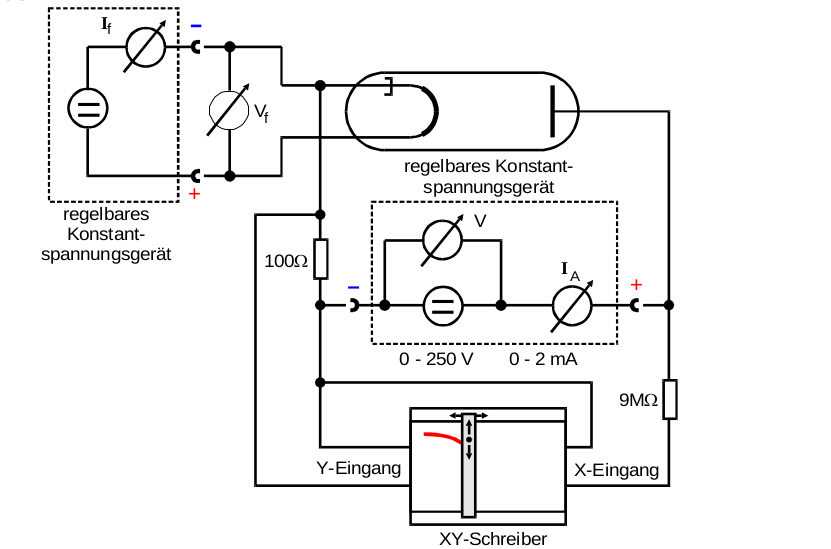
\includegraphics[height=7cm]{aufbau2.png}
  \caption{Versuchsaufbau zur Aufnahme von Kennlinien}
  \label{fig:aufbau2}
  \cite{skript}.
\end{figure}
